\documentclass[10pt,a4paper,oneside]{article}

\usepackage[utf8x]{inputenc}
\usepackage{amsmath}
\usepackage{amsfonts}
\usepackage{amssymb}
\usepackage{amsthm}
\usepackage{graphicx}
\usepackage[margin=0.75in]{geometry}
\usepackage{ucs}

\newcommand{\superscript}[1]{\ensuremath{^{\textrm{#1}}}}
\newcommand{\subscript}[1]{\ensuremath{_{\textrm{#1}}}}

\author{Michael Walker}
\title{Maths Problems: Triangle}

\begin{document}

\maketitle{}

Find x:

\begin{figure}[here]
  \begin{center}
    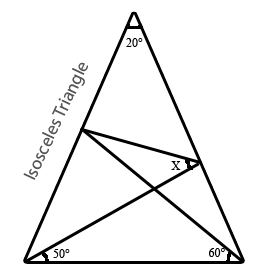
\includegraphics[scale=0.6]{problem.png}
    \caption{Isosceles Triangle}
    \label{fig:problem}
  \end{center}
\end{figure}

Solution on next page.

\pagebreak

\begin{figure}[here]
  \begin{center}
    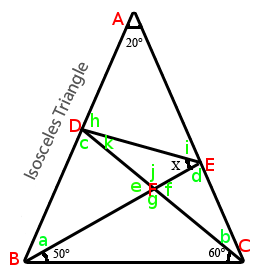
\includegraphics[scale=0.6]{solution.png}
    \caption{Isosceles Triangle}
    \label{fig:solution}
  \end{center}
\end{figure}

First, I wrote down everything obvious about the angles:
\begin{align*}
  g &= 70^\circ\\
  j &= 70^\circ\\
  e &= 110^\circ\\
  f &= 110^\circ\\
  a &= b + 10^\circ\\
  50 &= a + b\\
  \therefore b &= 20^\circ\\
  \therefore a &= 30^\circ\\
  d &= 50^\circ\\
  c &= 40^\circ\\
  k &= 110^\circ - x\\
  h &= 30^\circ + x\\
  i &= 130^\circ - x\\
\end{align*}

Then, I worked out all the sides using the sine and cosine rules
\begin{align*}
  BC &= \sqrt{2 - 2\textrm{cos} 20^\circ}\\
  BE &= \frac{BC \textrm{sin} 80^\circ}{\textrm{sin} 50^\circ}\\
  BF &= \frac{BC \textrm{sin} 60^\circ}{\textrm{sin} 70^\circ}\\
  CD &= \frac{BC \textrm{sin} 80^\circ}{\textrm{sin} 40^\circ}\\
  CF &= \frac{BC \textrm{sin} 50^\circ}{\textrm{sin} 70^\circ}\\
  CE &= \frac{CF \textrm{sin} 110^\circ}{\textrm{sin} 50^\circ}\\
  BD &= \frac{BF \textrm{sin} 110^\circ}{\textrm{sin} 40^\circ}\\
  DF &= \frac{BF \textrm{sin} 30^\circ}{\textrm{sin} 40^\circ}\\
  EF &= \frac{CF \textrm{sin} 20^\circ}{\textrm{sin} 50^\circ}\\
  DE &= \frac{DF \textrm{sin} 70^\circ}{\textrm{sin} x}\\
  DA &= \frac{DE \textrm{sin} (130^\circ - x)}{\textrm{sin} 20^\circ}\\
  EA &= \frac{DE \textrm{sin} (30^\circ + x)}{\textrm{sin} 20^\circ}\\
\end{align*}

I then took a closer look at triangle DFE:
\begin{align*}
  DE &= \sqrt{DF^2 + FE^2 - 2 \times DF \times FE \times \textrm{cos} 70^\circ}\\
  DF &\approx 0.24897\\
  FE &\approx 0.12641\\
  \therefore DE &\approx 0.23757\\\\
  DF^2 &= FE^2 + DE^2 - 2 \times FE \times DE \times \textrm{cos} x\\
  \textrm{cos} x &\approx 0.1737\\
  x &\approx 79.996^\circ\\
  x &= 80.0^\circ \textrm{ (3sf)}\\
\end{align*}

\textit{Quod erat faciendum.}
\end{document}